\section{Koalition}
\subsection{Overview}
%What is Koalition (as an LP and cryptocurrency)
%How does Koalition work wrt to points exchange
%to price stability
%For marketing, etc.
Koalition is a blockchain-based, decentralized loyalty program that aims to consolidate the myriad of existing and future loyalty programs into a single, vast interconnected and interoperable network. The individual LPs in the Koalition network are connected via a rewards-based unicurrency called \textit{KOA}, a price-stable cryptocurrency that enables frictionless exchange and redemption of rewards across the network. KOA boasts utility as well as usability as a stable coin, growing the crypto-economy as a liquid asset that users are more willing to use than typically deflationary cryptocurrencies. Consumers will not only be able to use KOA to pay for products and services across the Koalition network, they will also be able to exchange KOA freely among themselves and other entities on the network. This will enable a rich rewards-based economy that unlocks the value of brand loyalty.
%
\begin{figure}[h] % use "t!" to force the float to start the float at top of page
    \centering
        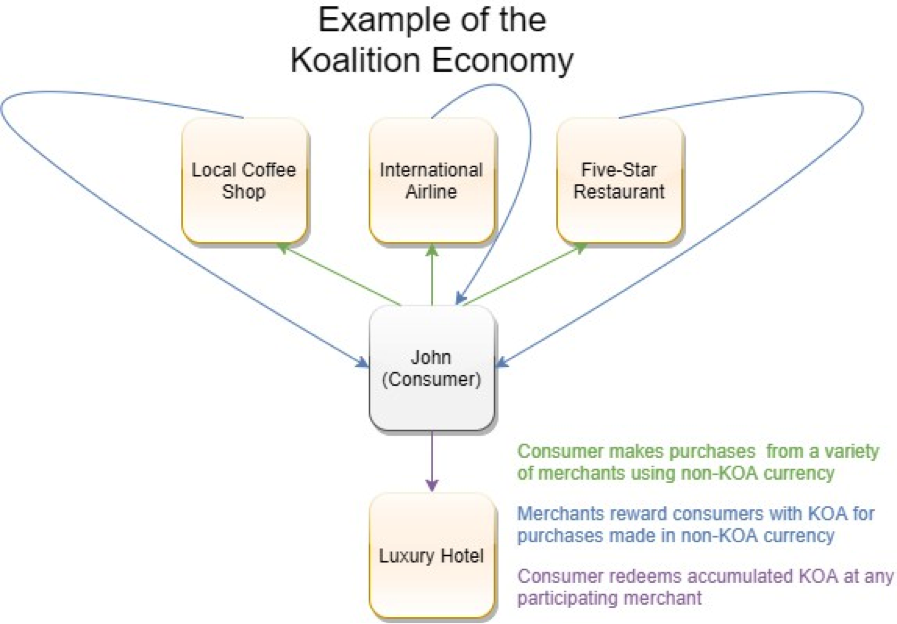
\includegraphics[keepaspectratio, width=0.7\textwidth]{images/KOAeconomy.png}
    \caption{The Koalition Economy} \label{fig:KOAeconomy}
\end{figure}

A paradigm shift in consumer behavioral and attitudinal loyalty has begun. Traditional stand-alone and coalition LPs have undoubtedly changed the dynamics of merchant competition and perpetuated the importance of relationship marketing. Koalition aims to satisfy customer demand through its vast network of merchants while maintaining integrity as a marketing tool for businesses by influencing customer buying behavior and perceptions through data analytics. Merchants now have the opportunity to embrace a disruptive technology that is bound to shake up the traditional LP economy. The following sections will discuss the intricacies of the Koalition protocol, specifically how it works, its limitations, and how it is bound to disrupt the loyalty programs space.

\subsection{Merchant Capabilities}

\subsubsection{Seamless Business Integration}
The Koalition loyalty program caters to the needs of all businesses selling products or services. From small local businesses to international corporations, each gain access to a network enhanced by blockchain technology. Small businesses gain access to a powerful marketing platform, opening their doors to a vast new customer acquisition and retention tool. Typically, small businesses do not have the infrastructure to build and support a robust LP. However, Koalition enables small businesses to integrate with current fiat payment options and will run effortlessly through autonomous contract execution. Furthermore, adopting cryptocurrencies as a means of payment eliminates large credit card transaction fees and delayed receipt of payments, which at times can be pivotal for small businesses.

For larger businesses, existing loyalty programs cannot be easily terminated from a marketing relationship perspective. Termination may be costly and negatively affect a company?s image. Fundamentally, customer relationship management as a corporate strategy creates high exit barriers \cite{Rehnen16}. Therefore, Koalition offers the flexibility of two different adoption options that cater to operational risk tolerance and perceived practicality of implementation.  


\begin{enumerate}
\item \textbf{Option 1: ``Koexist" with existing LPs} \\
Merchants can choose to keep their existing LP while offering consumers the option to pay for goods and services/receive rewards in KOA or the merchant?s native rewards currency. This non-invasive approach caters to businesses that have an existing LP that either wish to use both LPs indefinitely or are engineering a risk-averse exit strategy to their current LP.

\item \textbf{Option 2: Full Adoption of the Koalition Rewards Protocol} \\
Full adoption maximizes user utility for both merchants and consumers. Merchants who elect this option will replace all of the existing points in their current rewards program with KOA. The merchant must then choose how its customers who hold the native points can convert these to KOA (eg. convert cash value of native points to KOAs). Merchants who choose to fully adopt the Koalition Rewards Protocol will leverage the full extent of blockchain technology in the rewards economy. First, merchants will be fully integrated in a cooperative network where noncompetitive industries gain from each other. Second, liabilities akin to unredeemed rewards points become negligible as revenue is immediately realized.
\end{enumerate}

Streamlined onboarding of new partners perpetuates network effects. Koalition introduces an avenue for businesses of any size to partner with one another on one rewards network thus providing consumers with a convenient LP and introducing a paramount marketing opportunity to merchants. 
